\question
\tocsection{Three Pegs}

There is an infinite square grid of lattice points. There are three pegs on three corners of a square as shown in figure~\ref{fig:ThreePegsOnASquare_Problem}. A move consists of moving a peg over a peg to the opposite side, where the distance between the two pegs remains the same, as shown in figure~\ref{fig:ThreePegsOnASquare_MoveDefinition}.

\def\dotradius{0.05}
\def\pegradius{0.2}

\begin{figure}[H]
	\centering
	\begin{subfigure}{0.49\textwidth}
		\centering
		\begin{tikzpicture}[scale=0.8]
			\foreach \x in {0,1,...,7}{
				\foreach \y in {0,1,...,5}{
					\fill (\x,\y) circle (\dotradius);
				}
			}
			\fill[color=blue!60, blend mode=normal] (3,2) circle (\pegradius);
			\fill[color=blue!60, blend mode=normal] (3,3) circle (\pegradius);
			\fill[color=blue!60, blend mode=normal] (4,2) circle (\pegradius);
		\end{tikzpicture}
		\caption{Problem setup}
		\label{fig:ThreePegsOnASquare_Problem}
	\end{subfigure}
	\hfill
	\begin{subfigure}{0.49\textwidth}
		\centering
		\begin{tikzpicture}[scale=0.8]
			\foreach \x in {0,1,...,7}{
				\foreach \y in {0,1,...,5}{
					\fill (\x,\y) circle (\dotradius);
				}
			}
			\node[circle, draw, minimum size=\pegradius, color=blue!60] (A) at (4,0) {};
			\draw[->] (2,4) to [bend right=60] (A);
			\fill[color=blue!60, blend mode=normal] (3,2) circle (\pegradius);
			\fill[color=blue!60, blend mode=normal] (3,3) circle (\pegradius);
			\fill[color=blue!60, blend mode=normal] (2,4) circle (\pegradius);
			\draw[|<->|] ($(2,4)!0.15!(3,2)$) -- ($(2,4)!0.85!(3,2)$);
			\draw[|<->|] ($(3,2)!0.15!(4,0)$) -- ($(3,2)!0.85!(4,0)$);
		\end{tikzpicture}
		\caption{Example move}
		\label{fig:ThreePegsOnASquare_MoveDefinition}
	\end{subfigure}
	\caption{The three pegs on a square problem}
	\label{fig:ThreePegsOnASquare}
\end{figure}

\begin{parts}

\part \label{que:ThreePegsOnASquare_ConstantArea} Prove that the area of the triangle defined by the pegs is always $\frac{1}{2}$.

\begin{solution}

\begin{enumerate}
	\item There are many ways to find the area of a triangle, but the most useful formula to apply directly in this case is half the base times the height.
	\item Show that for an arbitrary move, the area before and after the move is preserved.
	\item Which edge of the triangle should be considered as the base?
\end{enumerate}

If peg~$i$ is jumped over peg~$j$, we define the base of the triangle to be the vector from peg~$i$ to peg~$j$. The altitude of the triangle is the perpendicular height to the third peg from the line that passes through pegs~$i$ and~$j$. After peg~$i$ has been moved, the altitude remains the same because peg~$i$ and peg~$j$ define the same line as before. The length of the base is also the same by definition of a move, and therefore the area is preserved.

\end{solution}

\part \label{que:ThreePegsOnASquare_LastCorner} Is it possible to move one of the pegs to the last corner of the square? Prove it is not possible or find the fewest moves to do so.

\begin{solution}

\begin{enumerate}
	\item Label the pegs $A$, $B$, and $C$. Label the points that a peg lands on with the name of the peg that landed there.
	\item Prove that the labelling in the previous hint is well-defined. That is, each square can only be landed on by a single type of peg. By labelling the fourth corner of the square as type $D$, deduce the conclusion.
	\item It is not possible.
	\item Consider the coordinates of a point before and after each move modulo 2.
\end{enumerate}

Define the four corners of the square as $A$, $B$, $C$, and $D$ with coordinates $(0, 0)$, $(1, 0)$, $(1, 1)$, and $(0, 1)$ respectively. Exploring with random moves and labelling the points where each peg lands, we may notice that we never need to give a point two different labels. This indicates some sort distinction between the pegs that is invariant and motivates understanding this invariant.

We call a point reachable by a peg starting on point $i$ as a point of type $i$. Our method of proof will be to show that this definition is well-defined, that is, each point has a unique type. This is equivalent to showing that a peg starting on a point with a given label cannot reach any point that is reachable by a peg starting on a point with a different label. Once this is fact has been established then we see that the last corner of the square cannot be reached as it is of type $D$ yet the initial pegs are of type $A$, $B$, and $C$.

If a peg with position vector $\mathbf{i}$ jumps over a peg with position vector $\mathbf{j}$ then the position vector of the point that the peg lands is $\mathbf{j} + (\mathbf{j} - \mathbf{i})$. By playing out a few moves and labelling the points with a type according to the rule defined previously, we hypothesize that the labels follow a pattern that repeats every two rows and every two columns. This motivates us to consider the coordinates modulo 2 as showing that two numbers are different modulo 2 is sufficient to show the two numbers are different. We apply this to our new position vector in~\eqref{eqn:ThreePegsOnASquare_PositionMod2}.
\begin{equation}
	\begin{alignedat}{2}
		& \mathbf{j} + (\mathbf{j} - \mathbf{i}) \quad && \mod 2 \\
		\equiv{} & 2\mathbf{j} - \mathbf{i} \quad && \mod 2 \\
		\equiv{} & \mathbf{i} \quad && \mod 2
	\end{alignedat}
	\label{eqn:ThreePegsOnASquare_PositionMod2}
\end{equation}

This shows that the position of a point of type $i$ modulo 2 is preserved. All of the initial pegs had different positions modulo 2, proving that a peg of type~$i$ can never land on a point of type~$j \ne i$. By our previous comments.

\end{solution}

\part \label{que:ThreePegsOnASquare_CharacteriseInitialProblem} For the starting configuration in figure~\ref{fig:ThreePegsOnASquare_Problem}, characterise (with proof) exactly which lattice points can be reached.

\begin{solution}

\begin{hints}

\begin{enumerate}
	\item The previous solution showed that the parity of a peg cannot change which limits the set of points that can be reached. It has not been proved that all points with the same parity can be reached.
	\item It is true that all points with the same parity can be reached.
	\item It is sufficient to show that the starting configuration can be moved two units in each of the cardinal directions.
\end{enumerate}

\end{hints}

In the solution presented to part~\ref{que:ThreePegsOnASquare_LastCorner} we hypothesized that the pattern of how points repeated every two units in each direction, but never proved this fact. We showed that the pattern could not repeat in any direction by any number not divisible by 2. The pattern does in fact repeat every two units. First we simplify the problem. Suppose that there exists a sequence of moves that results in the original pattern of three pegs being moved to the right by two units. The we make the following observations.

\begin{enumerate}
	\item There exists a mirror of symmetry that cuts diagonally through the original peg positions, therefore if the three pegs can be moved to the right by two units then they can be moved up by the same sequence performed when mirrored.
	\item The moves are reversible so if the pegs can move right by two then they can move left by two, and likewise for moving up and down by two.
	\item All $2 \times 2$ squares could therefore be reached by the original three pegs.
\end{enumerate}

All that is left to do is come up with such a sequence that moves the initial configuration to the right by two units. In fact, by the symmetries in our argument, finding a sequence that moves the initial configuration in any cardinal direction by two units would be sufficient. This can be done in four moves as follows where we assume the pegs are at (0, 0), (0, 1), and (1, 0), and is presented in figure~\ref{fig:ThreePegsOnASquare_MoveInitialConfiguration}.

\begin{enumerate}
	\item Move the peg at (0, 1) over the peg at (1, 0) to (2, -1).
	\item Move the peg at (0, 0) over the peg at (1, 0) to (2, 0). 
	\item Move the peg at (1, 0) over the peg at (2, 0) to (3, 0).
	\item Move the peg at (2, -1) over the peg at (2, 0) to (2, 1).
\end{enumerate}


\begin{figure}[H]
	\begin{subfigure}{0.24\textwidth}
		\centering
		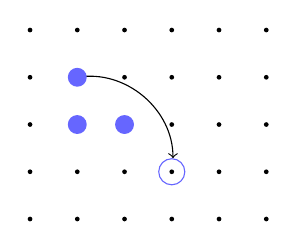
\begin{tikzpicture}[scale=0.6]
			\foreach \x in {1,2,...,6}{
				\foreach \y in {0,1,...,4}{
					\fill (\x,\y) circle (\dotradius);
				}
			}
			\node[circle, draw, minimum size=\pegradius, color=blue!60, blend mode=normal] (A) at (4,1) {};
			\draw[->] (2,3) to [bend left=50] (A);
			\fill[color=blue!60, blend mode=normal] (2,2) circle (\pegradius);
			\fill[color=blue!60, blend mode=normal] (2,3) circle (\pegradius);
			\fill[color=blue!60, blend mode=normal] (3,2) circle (\pegradius);
			
		\end{tikzpicture}
		\caption{Move 1}
	\end{subfigure}
	\hfill
	\begin{subfigure}{0.24\textwidth}
		\centering
		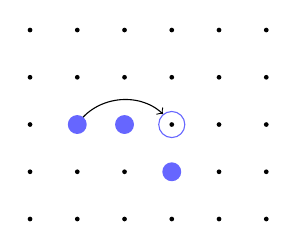
\begin{tikzpicture}[scale=0.6]
			\foreach \x in {1,2,...,6}{
				\foreach \y in {0,1,...,4}{
					\fill (\x,\y) circle (\dotradius);
				}
			}
			\node[circle, draw, minimum size=\pegradius, color=blue!60, blend mode=normal] (A) at (4,2) {};
			\draw[->] (2,2) to [bend left=50] (A);
			\fill[color=blue!60, blend mode=normal] (2,2) circle (\pegradius);
			\fill[color=blue!60, blend mode=normal] (4,1) circle (\pegradius);
			\fill[color=blue!60, blend mode=normal] (3,2) circle (\pegradius);
			
		\end{tikzpicture}
		\caption{Move 2}
	\end{subfigure}
	\begin{subfigure}{0.24\textwidth}
		\centering
		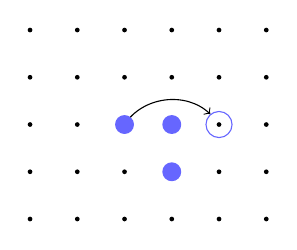
\begin{tikzpicture}[scale=0.6]
			\foreach \x in {1,2,...,6}{
				\foreach \y in {0,1,...,4}{
					\fill (\x,\y) circle (\dotradius);
				}
			}
			\node[circle, draw, minimum size=\pegradius, color=blue!60, blend mode=normal] (A) at (5,2) {};
			\draw[->] (3,2) to [bend left=50] (A);
			\fill[color=blue!60, blend mode=normal] (4,2) circle (\pegradius);
			\fill[color=blue!60, blend mode=normal] (4,1) circle (\pegradius);
			\fill[color=blue!60, blend mode=normal] (3,2) circle (\pegradius);
			
		\end{tikzpicture}
		\caption{Move 3}
	\end{subfigure}
	\hfill
	\begin{subfigure}{0.24\textwidth}
		\centering
		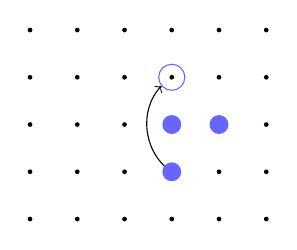
\begin{tikzpicture}[scale=0.6]
			\foreach \x in {1,2,...,6}{
				\foreach \y in {0,1,...,4}{
					\fill (\x,\y) circle (\dotradius);
				}
			}
			\node[circle, draw, minimum size=\pegradius, color=blue!60, blend mode=normal] (A) at (4,3) {};
			\draw[->] (4,1) to [bend left=50] (A);
			\fill[color=blue!60, blend mode=normal] (4,2) circle (\pegradius);
			\fill[color=blue!60, blend mode=normal] (4,1) circle (\pegradius);
			\fill[color=blue!60, blend mode=normal] (5,2) circle (\pegradius);
			
		\end{tikzpicture}
		\caption{Move 4}
	\end{subfigure}
	\caption{Moving the initial configuration to the right by two units.}
	\label{fig:ThreePegsOnASquare_MoveInitialConfiguration}
\end{figure}

\end{solution}

\part \label{que:ThreePegsOnASquare_CharacteriseHigherDimensional} Consider the higher-dimensional analague of part~\ref{que:ThreePegsOnASquare_CharacteriseInitialProblem}. On an $n$-dimensional infinite lattice there are pegs at the origin and one unit along each of the coordinate axes. Explicitly we have $v_0 = (0, \dots, 0)$ and $v_k = (0, \dots, 0, 1, 0, \dots, 0)$ where the 1 occurs in the $k$th position for $k = 1, \dots, n$. Using your answers from parts~\ref{que:ThreePegsOnASquare_LastCorner} and~\ref{que:ThreePegsOnASquare_CharacteriseInitialProblem} or otherwise, characterise (with proof) exactly which lattice points can be reached for this starting configuration.

\begin{hints}
	
	\begin{enumerate}
		\item This is very similar to the earlier parts. This question is only testing whether you are capable of abstracting.
		\item Can you move one point at a time?
		\item Consider the origin, a point in the cardinal direction you want to move, and another point. This defines a plane and the problem is exactly the same as the two-dimensional variant, expect the first two points need to end up in the same position they started in after any sequence of moves.
	\end{enumerate}
	
\end{hints}

\begin{solution}

The proof in part~\ref{que:ThreePegsOnASquare_LastCorner} is independent of dimension\footnote{It even works in infinitely many dimensions.} so again we see that the coordinates of our points modulo 2 is invariant. This has characterised some points as definitely unreachable, but we still need to prove that the remaining points are reachable. The proof from part~\ref{que:ThreePegsOnASquare_CharacteriseInitialProblem} can be modified to work for this higher dimensional configuration.

Pick a direction to move along, let us say along the $k$th axis, we show that all the other points can be moved by two units in this direction. We look at each $v_i$ where $i \ne k$ and show how to move that point by two units. Looking at the plane passing through the origin, $v_k$, and $v_i$, we see we are in exactly the same situation as part~\ref{que:ThreePegsOnASquare_CharacteriseInitialProblem} and therefore the same sequence of moves can be applied.

The peg now at $3v_k$ can jump over the peg now at $2v_k$ to land at $v_k$ where it started. Similarly the peg at $v_2$ can jump over the peg at $v_k$ to land back at the origin. This situation is now identical to the starting configuration, apart from the peg that started at $v_i$ has been moved to $v_i + 2v_k$. We can repeat this for all $i \ne k$, and if the last two ``undoing moves" are not done then the origin and $v_k$ are also moved two units right, meaning the whole configuration has been moved. This procedure is actually more complicated than it needs to be, and we will see an even simpler method of moving points in part~\ref{que:ThreePegsOnASquare_CharacteriseSpecialCase}.

\end{solution}

\part \label{que:ThreePegsOnASquare_CharacteriseSpecialCase} Consider a three-dimensional infinite lattice with pegs at $(1, 0, 0)$, $(0, 1, 0)$, and $(0, 0, 1)$. How does the characterisation of reachable lattice points differ from part~\ref{que:ThreePegsOnASquare_CharacteriseHigherDimensional}? Hence conjecture what the characterisation might be for any starting configuration of pegs on an $n$-dimensional infinite lattice. Can you prove this?

\begin{solution}

We cannot do the same proof as in part~\ref{que:ThreePegsOnASquare_CharacteriseHigherDimensional} because we no longer have a peg at the origin. The three pegs define the plane and all moves keep the pegs within that plane. This is because the vector that each peg moves by is necessarily contained within the plane by definition of a move. If we restrict the lattice to only the points contained within the same plane as the pegs then we see they form a two-dimensional lattice. The same result as in part~\ref{que:ThreePegsOnASquare_CharacteriseInitialProblem} gives the characterisation in this case, but restricted to this new lattice.

Looking towards generalising this to any configuration of points, we extend this observation to get a restriction on what points are reachable. Reachable points must lie within the space that the vectors that connect each pair of points can cover when starting from one of the pegs. More formally, if $V$ is the set of differences between the position vectors of the pegs and $v$ is the position vector of an arbitrary peg, then the set of reachable points must be a subset of $R = \{v + \sum_i^N \alpha_i v_i | \alpha_i \in \mathbb{Z}, v_i \in V, n \in \mathbb{N} \}$\footnote{All finite linear combinations of $v_i \in V$ is referred to as the span of $V$ and is a vector space. $R = v + \operatorname{span}{U}$ is known as an affine space.}.

We also know that the coordinates must preserve the parity of the original pegs. Based on the intuition we have built up so far, we conjecture that the points in $R$ that have the same parity as one of the original pegs are the reachable points. To prove this we can emulate the proof from part~\ref{que:ThreePegsOnASquare_CharacteriseHigherDimensional}. It is sufficient to show that for any initial peg positions $v_i$ and $v_j$, any other peg can be moved by $2(v_i - v_j)$ while leaving the other pegs unchanged. The factor of two is needed to preserve parity.

We prove this for the simpler case where all pegs have different parity. Without loss of generality, we consider three pegs $P_1$, $P_2$, and $P_3$ with position vectors $v_1$, $v_2$, and $v_3$, and we attempt to move $v_3$ by $2(v_2 - v_1)$ with the pegs at $v_1$ and $v_2$ returning to their original positions. All our moves here are well-defined as a peg cannot land on another peg due to having different parities. If $P_3$ jumps over $P_1$ then over $P_2$ then it initially moves to $v_1 + (v_1 - v_3) = 2v_1 - v_3$, then to $v_2 + (v_2 - (2v_1 - v_3)) = v_3 + 2(v_2 - v_1)$.

The general case where pegs can have the same parity is more complicated, but we can apply a similar idea to the simple case. If we cannot jump peg $P_3$ over $P_1$ we can move $P_1$ or $P_2$ and try again, let us say we jump $P_1$ over $P_2$ and relabel it peg $P'_1$. We can apply the same method as before but with pegs $P_2$ and $P'_1$ instead of pegs $P_1$ and $P_2$. The vector from $P_1$ to $P_2$ is the same as the vector from $P_2$ to $P'_1$ so $P_3$ will be moved by the same amount. If this does not work then we can keep jumping pegs $P_1$ and $P_2$ over each other until they are far away.

We still need to prove that this process works and is always possible. There are potential problems.
\begin{enumerate}
	\item Is this process of flipping $P_1$ and $P_2$ guaranteed to work after finitely many time steps? That is, could we get stuck in a loop where no matter how many times we flip $P_1$ and $P_2$ over each other, there is always some other peg that gets in the way.
	\item Can we always flip $P_1$ and $P_2$ over each other?
\end{enumerate}

If we have finitely many pegs, let us say $n$, then the answer to the first statement is yes. After each flip of $P_1$ and $P_2$, the result of flipping $P_3$ over each of $P_1$ and $P_2$ must be different. This means that after $2n$ total flips, alternating between $P_1$ and $P_2$, we must have reached some state where all moves involving $P_3$ were well-defined by the pigeonhole principle. $P_1$ and $P_2$ can then retrace their steps and return to their original positions.

For $P_1$ not to be able to flip over $P_2$ there must exist some peg, $P_4$ that is an equal distance away from $P_2$ as $P_1$ but in the opposite direction. If this is the case then we can use $P_2$ and $P_4$ instead of $P_1$ and $P_2$ as they necessarily have the same vector between them.

The situation with infinitely many pegs or pegs on an infinite dimensional lattice is more complicated due to potential issues about convergence and is therefore not covered here. We note that having infintely many pegs does not necessarily make the situation more complicated. Consider a one-dimensional lattice with pegs at even-numbered positions and one peg at an odd-numbered position - here it is clear that all points are reachable.

\end{solution}

\end{parts}